\chapter{消息框}
PyAutoGUI 利用 PyMsgBox 中的消息框函数，提供了一种跨平台、纯 Python 的方式来显示类似 JavaScript 的消息框。总共提供了四种消息框函数：
\begin{enumerate}[label=\arabic*)]
    \item \codeinline{alert()}：显示一个简单的消息框，只有一个“确定”按钮。
    \item \codeinline{confirm()}：显示一个确认消息框，包含“确定”和“取消”按钮。
    \item \codeinline{prompt()}：显示一个输入消息框，包含“确定”和“取消”按钮。
    \item \codeinline{password()}：显示一个密码输入消息框，包含“确定”和“取消”按钮。
\end{enumerate}

\section{alert() 消息框}
\codeinline{alert()} 函数显示一个简单的消息框，只有一个“确定”按钮。
\begin{lstlisting}[style=demostyle,numbers=none]
# text 是消息框中显示的文本
# title 是消息框的标题, 默认 'Alert'
# buttons 是消息框中显示的按钮文本, 默认 'OK'
pyautogui.alert(text)
>> pyautogui.alert('Hello world!')
>> pyautogui.alert('Hello world!', 'Title')
>> pyautogui.alert('Hello world!', 'Title', 'OK')
# 返回值是用户点击的按钮文本, 只有一个按钮时返回 'OK'
# 如果用户点击了“确定”按钮，则返回 'OK'
return 'OK'
\end{lstlisting}

\begin{figure}[htpb]
    \centering
    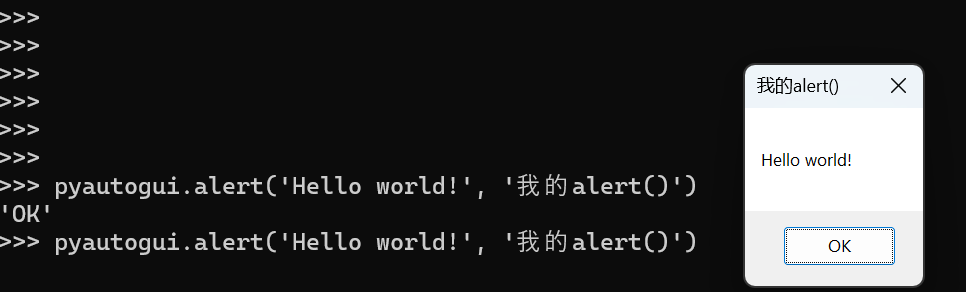
\includegraphics[width=0.4\textwidth]{part/图形化/pyautogui/pic/消息框/alert消息框.png}
    \caption{alert消息框}
\end{figure}


\section{confirm() 确认消息框}
\codeinline{confirm()} 函数显示一个确认消息框，包含“确定”和“取消”按钮。
\begin{lstlisting}[style=demostyle,numbers=none]
# text 是消息框中显示的文本
# title 是消息框的标题, 默认 'Confirm'
# buttons 是消息框中显示的按钮文本, 默认 'OK', 'Cancel'
pyautogui.confirm(text, title, buttons)

>>> pyautogui.confirm('Are you sure you want to continue?')
>>> pyautogui.confirm('Are you sure you want to continue?', 'Title')
>>> pyautogui.confirm('Are you sure you want to continue?', 'Title', ['Yes', 'No'])
# 返回值是用户点击的按钮文本, 如果用户点击了“确定”按钮，则返回 'OK'
# 如果用户点击了“取消”按钮，则返回 'Cancel'
return 'OK' or 'Cancel'
\end{lstlisting}

\begin{figure}[htpb]
    \centering
    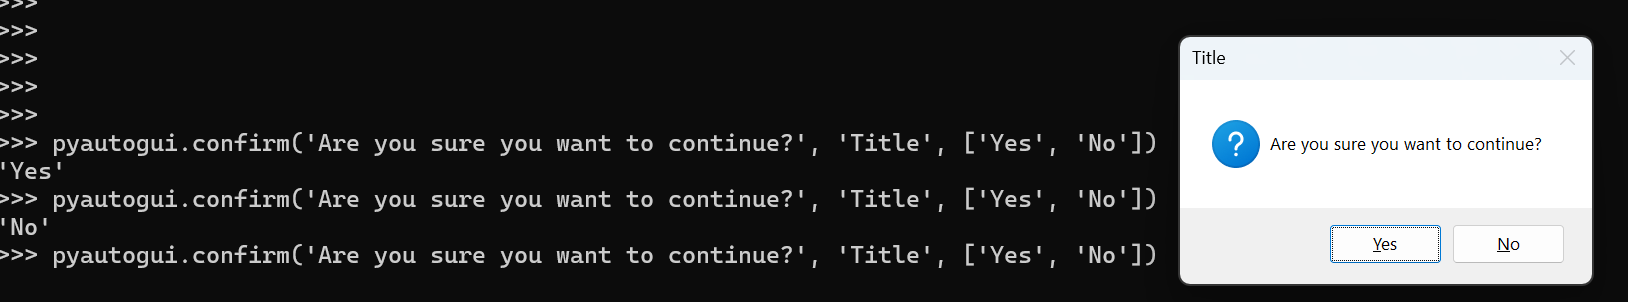
\includegraphics[width=0.4\textwidth]{part/图形化/pyautogui/pic/消息框/confirm消息框.png}
    \caption{confirm消息框}
\end{figure}

\section{prompt() 输入消息框}
\codeinline{prompt()} 函数显示一个输入消息框，包含“确定”和“取消”按钮。
\begin{lstlisting}[style=demostyle,numbers=none]    
# text 是消息框中显示的文本
# title 是消息框的标题, 默认 'Prompt'
# default 是输入框中的默认文本, 默认 ''
pyautogui.prompt(text, title, default)

>>> pyautogui.prompt('What is your name?')
>>> pyautogui.prompt('What is your name?', 'Title')
>>> pyautogui.prompt('What is your name?', 'Title', 'Default Name')
\end{lstlisting}

\begin{figure}[htpb]
    \centering
    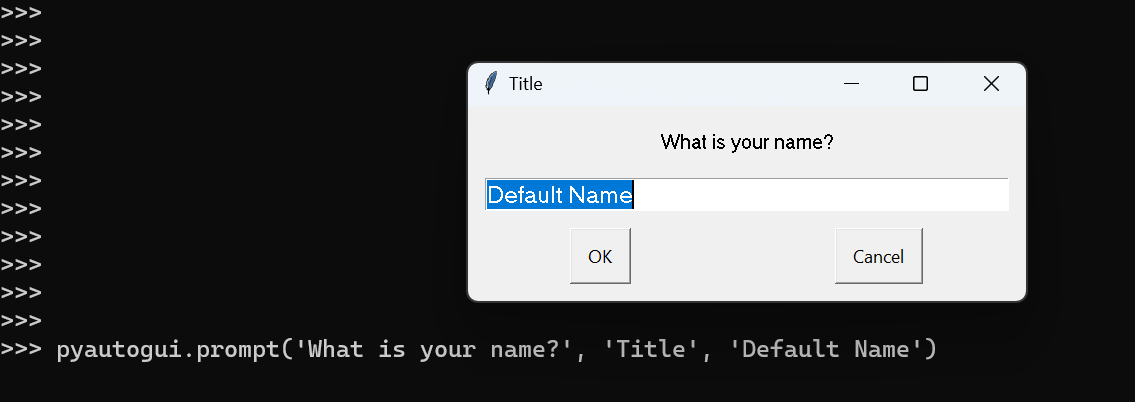
\includegraphics[width=0.4\textwidth]{part/图形化/pyautogui/pic/消息框/prompt消息框.png}
    \caption{prompt消息框}
\end{figure}


\section{password() 密码输入消息框}
\codeinline{password()} 函数显示一个密码输入消息框，包含“确定”和“取消”按钮。
\begin{lstlisting}[style=demostyle,numbers=none]
# text 是消息框中显示的文本
# title 是消息框的标题, 默认 'Password'
# default 是输入框中的默认文本, 默认 ''
# mask 是输入框中显示的掩码字符, 默认 '*'
pyautogui.password(text, title, default, mask)

>>> pyautogui.password('Enter your password:')
>>> pyautogui.password('Enter your password:', 'Title')
>>> pyautogui.password('Enter your password:', 'Title', 'Default Password')
>>> pyautogui.password('Enter your password:', 'Title', 'Default Password', '#')
# 返回值是用户输入的密码文本, 如果用户点击了“取消”按钮，则返回 None
return 'password' or None   
\end{lstlisting}

\begin{figure}[htpb]
    \centering
    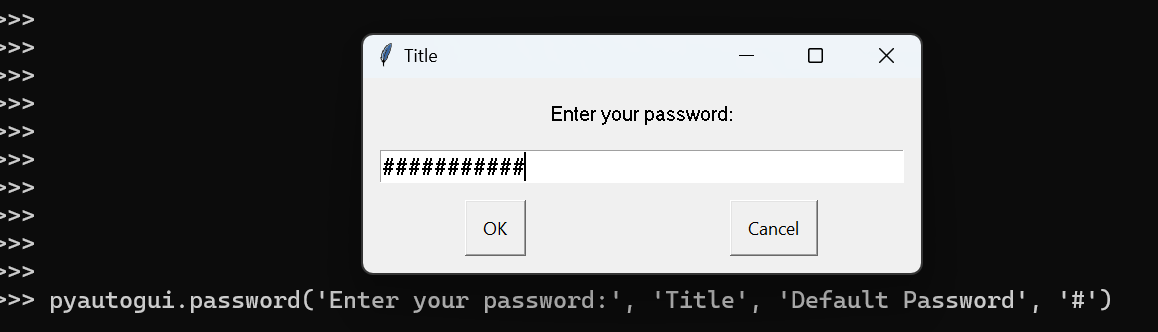
\includegraphics[width=0.4\textwidth]{part/图形化/pyautogui/pic/消息框/password消息框.png}
    \caption{password消息框}
\end{figure}

